\documentclass[border=15pt, multi, tikz]{standalone}
\usepackage{import}
\usepackage{ctex}% 中文支持
\usepackage{tikz}

\subimport{../}{init}
\usetikzlibrary{positioning}
\usetikzlibrary{3d} %for including external image
\usetikzlibrary{quotes,angles}
\usetikzlibrary{calc}
\usetikzlibrary{decorations.pathreplacing}

\def\DataColor{rgb:blue,5;white,5}
\def\ConvColor{rgb:yellow,5;red,2.5;white,5}
\def\ConvReluColor{rgb:yellow,5;red,5;white,5}
\def\PoolColor{rgb:red,1;black,0.3}
\def\PcColor{rgb:blue,5;red,2.5;white,5}
\def\PcSquashColor{rgb:blue,5;red,5;white,4}
\def\DcColor{rgb:blue,5;green,15}
\def\SumColor{rgb:blue,5;green,15}
% \def\SoftmaxColor{rgb:magenta,5;black,7}

\begin{document}
\begin{tikzpicture}
%%%%%%%%%%%%%%%%%%%%%%%%%%%%%%%
% 图像大小
%%%%%%%%%%%%%%%%%%%%%%%%%%%%%%%

\tikzstyle{connection}=[ultra thick,every node/.style={sloped,allow upside down},draw=\edgecolor,opacity=0.7]
%%%%%%%%%%%%%%%%%%%%%%%%%%%%%%%%%%%%%%%%%%%%%%%%%%%%%%%%%%%%%%%%%%%%%%%%%%%%%%%%%%%%%%%%
%% Data
%%%%%%%%%%%%%%%%%%%%%%%%%%%%%%%%%%%%%%%%%%%%%%%%%%%%%%%%%%%%%%%%%%%%%%%%%%%%%%%%%%%%%%%%
\node[canvas is zy plane at x=0] (state) at (-4.5,0,0) {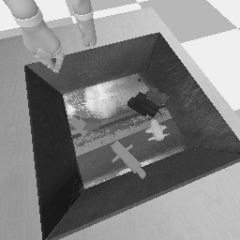
\includegraphics[width=6cm,height=6cm]{observation.png}};
maxpool
% \pic[shift={(-5,0,0)}] at (0,0,0) {Box={name=obs,fill=\DataColor,opacity=0.5,height=32,width=2,depth=32}};
%%%%%%%%%%%%%%%%%%%%%%%%%%%%%%%%%%%%%%%%%%%%%%%%%%%%%%%%%%%%%%%%%%%%%%%%%%%%%%%%%%%%%%%%
%% 卷积单元
%%%%%%%%%%%%%%%%%%%%%%%%%%%%%%%%%%%%%%%%%%%%%%%%%%%%%%%%%%%%%%%%%%%%%%%%%%%%%%%%%%%%%%%%
%% Conv1
\pic[shift={(6,0,0)}] at (state) {RightBandedBox={name=cr1,%
        xlabel={{"128", "128"}},ylabel=126,zlabel=126,fill=\ConvColor,bandfill=\ConvReluColor,%
        height=60,width=20,depth=60}};
%% Conv2
\pic[shift={(5,0,0)}] at (cr1-east) {RightBandedBox={name=cr2,%
        xlabel={{"64", "64"}},ylabel=124,zlabel=124,fill=\ConvColor,bandfill=\ConvReluColor,%
        height=50,width=12,depth=50}};
%% Conv3
\pic[shift={(4,0,0)}] at (cr2-east) {RightBandedBox={name=cr3,%
        xlabel={{"64", "64"}},ylabel=122,zlabel=122,fill=\ConvColor,bandfill=\ConvReluColor,%
        height=40,width=8,depth=40}};
% maxpool
\pic[shift={(3,0,0)}] at (cr3-east) {Box={name=p1,fill=\PoolColor,opacity=0.5,height=30,width=2,depth=30}};
% 注释
\node[shift={(-4.5, -9.5, 0)}] at (cr1-east) {卷积层1};
\node[shift={(-2.5, -8, 0)}] at (cr2-east) {卷积层2};
\node[shift={(-2.5, -7, 0)}] at (cr3-east) {卷积层3};
\node[shift={(-1.5, -5, 0)}] at (p1-east) {池化层1};
% 卷积单元之间的连接
\draw [connection]  (state) -- node {\midarrow} (cr1-west);
\draw [connection]  (cr1-east) -- node {\midarrow} (cr2-west);
\draw [connection]  (cr2-east) -- node {\midarrow} (p1-west);
% 卷积单元的注释
\coordinate (point1) at ([shift={(0, -9, 0)}] p1-east);
\coordinate (point2) at ([shift={(-2, -9, 0)}] cr1-west);
\draw[decorate, decoration={brace, raise=15pt,amplitude=0.7cm}] (point1) -- (point2);
\node[shift={(-2.3, -10.6, 0)}] at (cr2-east) {卷积单元};
%%%%%%%%%%%%%%%%%%%%%%%%%%%%%%%%%%%%%%%%%%%%%%%%%%%%%%%%%%%%%%%%%%%%%%%%%%%%%%%%%%%%%%%%
%% 卷积单元需要乘以2
%%%%%%%%%%%%%%%%%%%%%%%%%%%%%%%%%%%%%%%%%%%%%%%%%%%%%%%%%%%%%%%%%%%%%%%%%%%%%%%%%%%%%%%%
\node[shift={(4, 0, 0)}, canvas is xy plane at z=0] (ellipsis1) at (p1-east) {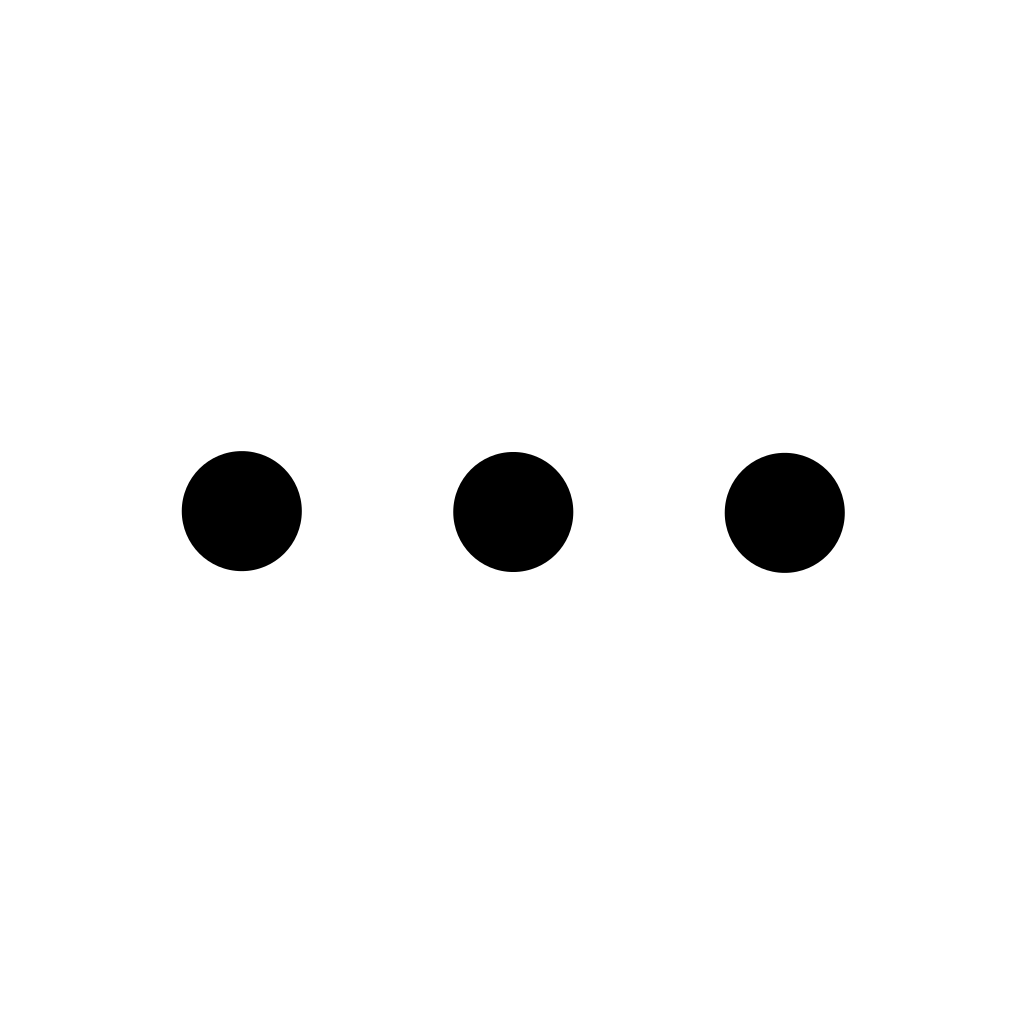
\includegraphics[width=2cm,height=2cm]{../cellipsis.png}};
\node[shift={(2, 0, 0)}, canvas is xy plane at z=0] (temp) at (ellipsis1) {
\includegraphics[width=2cm,height=2cm]{../x2.png}};
\node[shift={(2, 0, 0)}, canvas is xy plane at z=0] (ellipsis2) at (temp) {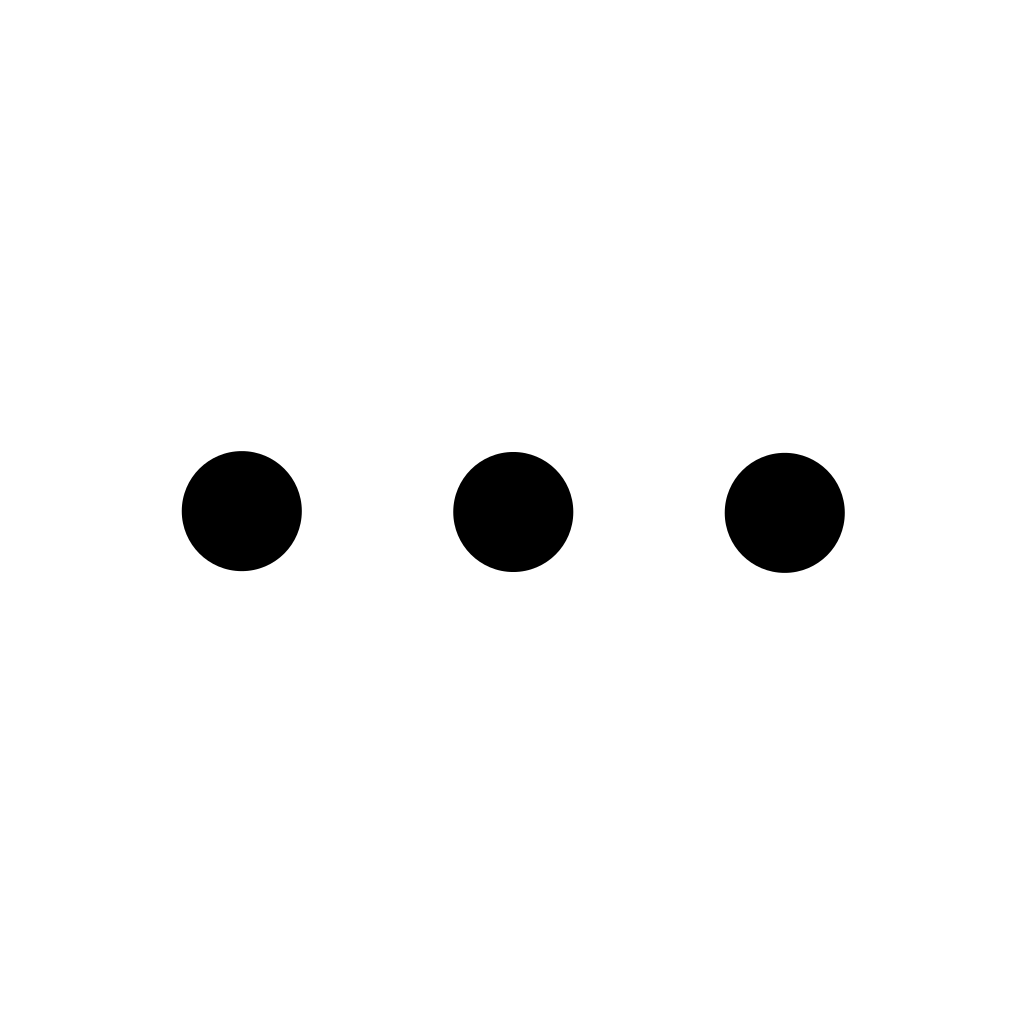
\includegraphics[width=2cm,height=2cm]{../cellipsis.png}};
\draw [connection]  (p1-east) -- node {\midarrow} (ellipsis1);
% 卷积栈
\coordinate (point3) at ([shift={(0, -10, 0)}] ellipsis2);
\coordinate (point4) at ([shift={(-2, -10, 0)}] cr1-west);
\draw[decorate, decoration={brace, raise=15pt,amplitude=0.7cm}] (point3) -- (point4);
\node[shift={(1.7, -11.5, 0)}] at (cr2-east) {卷积栈};
%%%%%%%%%%%%%%%%%%%%%%%%%%%%%%%%%%%%%%%%%%%%%%%%%%%%%%%%%%%%%%%%%%%%%%%%%%%%%%%%%%%%%%%%
%% 卷积单元
%%%%%%%%%%%%%%%%%%%%%%%%%%%%%%%%%%%%%%%%%%%%%%%%%%%%%%%%%%%%%%%%%%%%%%%%%%%%%%%%%%%%%%%%
%% Conv1
\pic[shift={(2.5,0,0)}] at (ellipsis2) {RightBandedBox={name=cr3,%
        xlabel={{"16", "16"}},ylabel=26,zlabel=26,fill=\ConvColor,bandfill=\ConvReluColor,%
        height=18,width=5,depth=18}};
%% Conv2
\pic[shift={(2,0,0)}] at (cr3-east) {RightBandedBox={name=cr4,%
        xlabel={{"16", "16"}},ylabel=24,zlabel=24,fill=\ConvColor,bandfill=\ConvReluColor,%
        height=15,width=5,depth=15}};

% 注释
\node[shift={(-1, -3.5, 0)}] at (cr3-east) {卷积层7};
\node[shift={(-1.5, -3, 0)}] at (cr4-east) {卷积层8};
% 卷积单元之间的连接
\draw [connection]  (ellipsis2)        -- node {\midarrow} (cr3-west);
\draw [connection]  (cr3-east)        -- node {\midarrow} (cr4-west);
%%%%%%%%%%%%%%%%%%%%%%%%%%%%%%%%%%%%%%%%%%%%%%%%%%%%%%%%%%%%%%%%%%%%%%%%%%%%%%%%%%%%%%%%
%% Linear Layer1
%%%%%%%%%%%%%%%%%%%%%%%%%%%%%%%%%%%%%%%%%%%%%%%%%%%%%%%%%%%%%%%%%%%%%%%%%%%%%%%%%%%%%%%%
\pic[shift={(4,0,0)}] at (cr4-east) {RightBandedBox={name=fc1-1,
        fill=\PcColor,bandfill=\PcSquashColor,%
        height=8,width=3,depth=3}};
% 平移
\pic[shift={(4,0,4)}] at (cr4-east) {RightBandedBox={name=fc1-2,
        fill=\PcColor,bandfill=\PcSquashColor,%
        height=8,width=3,depth=3}};
\pic[shift={(4,0,4+2)}] at (cr4-east) {RightBandedBox={name=fc1-3,
        fill=\PcColor,bandfill=\PcSquashColor,%
        height=8,width=3,depth=3}};
\pic[shift={(4,0,4+4)}] at (cr4-east) {RightBandedBox={name=fc1-4,
        fill=\PcColor,bandfill=\PcSquashColor,%
        height=8,width=3,depth=3}};
\pic[shift={(4,0,4+6)}] at (cr4-east) {RightBandedBox={name=fc1-5,
        fill=\PcColor,bandfill=\PcSquashColor,%
        height=8,width=3,depth=3}};

\pic[shift={(4,0,-4)}] at (cr4-east) {RightBandedBox={name=fc1-6,
        fill=\PcColor,bandfill=\PcSquashColor,%
        height=8,width=3,depth=3}};
\pic[shift={(4,0,-4-2)}] at (cr4-east) {RightBandedBox={name=fc1-7,
        fill=\PcColor,bandfill=\PcSquashColor,%
        height=8,width=3,depth=3}};
\pic[shift={(4,0,-4-4)}] at (cr4-east) {RightBandedBox={name=fc1-8,
        fill=\PcColor,bandfill=\PcSquashColor,%
        height=8,width=3,depth=3}};
\pic[shift={(4,0,-4-6)}] at (cr4-east) {RightBandedBox={name=fc1-9,
        fill=\PcColor,bandfill=\PcSquashColor,%
        height=8,width=3,depth=3}};
% 省略号
\node[shift={(0, 0, 2.7)}, canvas is zy plane at x=0] (temp) at (fc1-1-east) {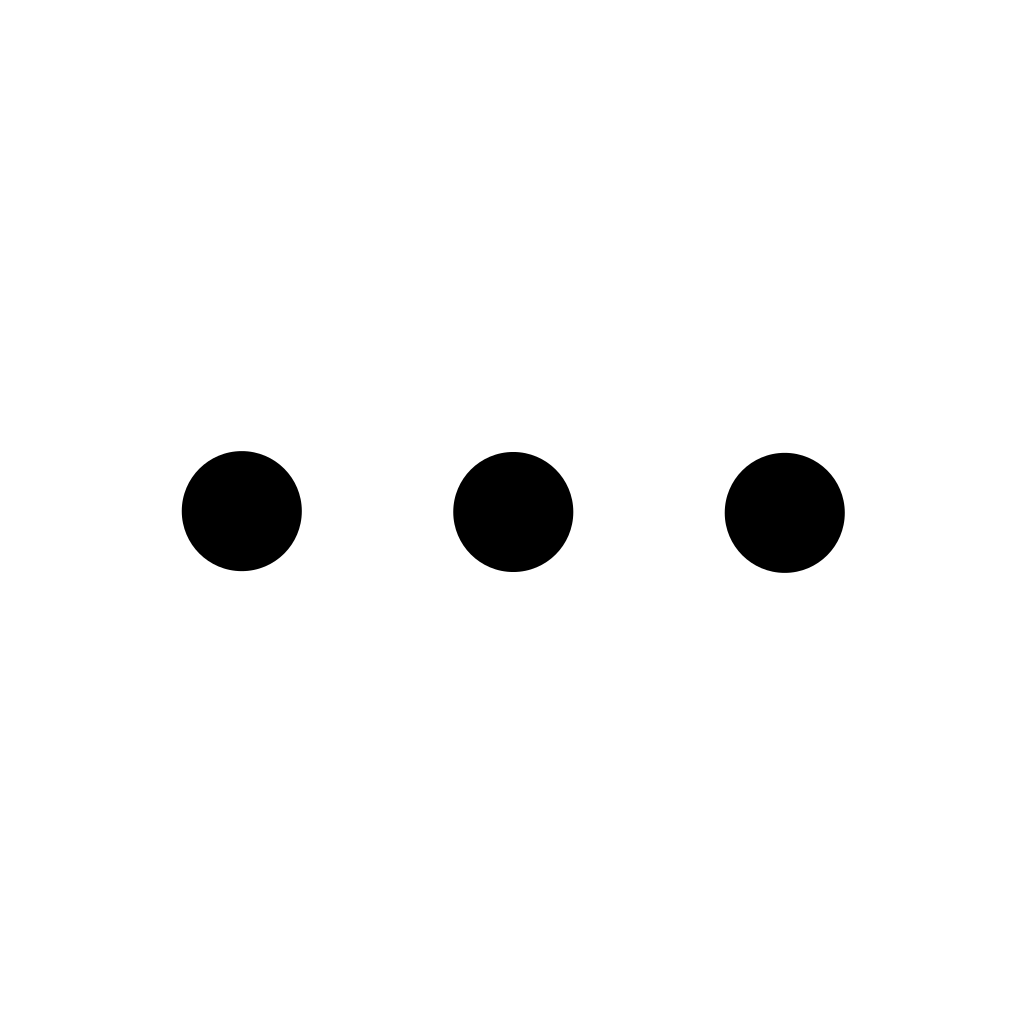
\includegraphics[width=2cm,height=2cm]{../cellipsis.png}};
\node[shift={(0, 0, -1.2)}, canvas is zy plane at x=0] (temp) at (fc1-1-east) {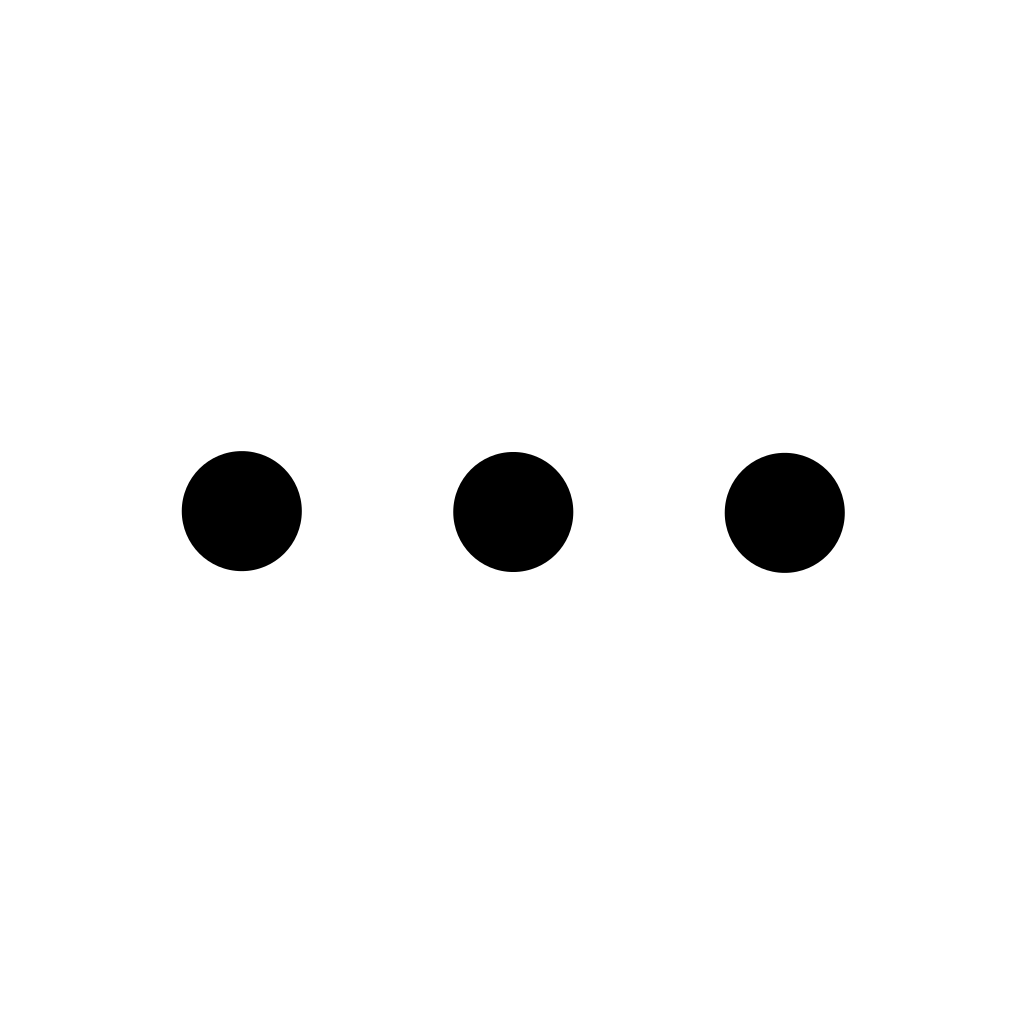
\includegraphics[width=2cm,height=2cm]{../cellipsis.png}};
%%%%%%%%%%%%%%%%%%%%%%%%%%%%%%%%%%%%%%%%%%%%%%%%%%%%%%%%%%%%%%%%%%%%%%%%%%%%%%%%%%%%%%%%
%% Draw Dotted Edges
%%%%%%%%%%%%%%%%%%%%%%%%%%%%%%%%%%%%%%%%%%%%%%%%%%%%%%%%%%%%%%%%%%%%%%%%%%%%%%%%%%%%%%%%
\draw[densely dashed]
    (fc1-5-west)++(3, 3.7, 8) coordinate(a) -- (cr4-nearnortheast)
    (fc1-5-west)++(2, 1.3, 5.5) coordinate(b) -- (cr4-nearsoutheast)
    (fc1-9-west)++(-0.5, -1.9, -3) coordinate(c) -- (cr4-farsoutheast)
    (fc1-9-west)++(0, 1, 0) coordinate(d) -- (cr4-farnortheast)
    ;
%%%%%%%%%%%%%%%%%%%%%%%%%%%%%%%%%%%%%%%%%%%%%%%%%%%%%%%%%%%%%%%%%%%%%%%%%%%%%%%%%%%%%%%%
%% Linear Layer2
%%%%%%%%%%%%%%%%%%%%%%%%%%%%%%%%%%%%%%%%%%%%%%%%%%%%%%%%%%%%%%%%%%%%%%%%%%%%%%%%%%%%%%%%
% 平移
\pic[shift={(12,0,2)}] at (fc1-1-east) {RightBandedBox={name=fc2-1,
        fill=\PcColor,bandfill=\PcSquashColor,%
        height=8,width=3,depth=3}};
\pic[shift={(12,0,2+2)}] at (fc1-1-east) {RightBandedBox={name=fc2-2,
        fill=\PcColor,bandfill=\PcSquashColor,%
        height=8,width=3,depth=3}};
\pic[shift={(12,0,2+4)}] at (fc1-1-east) {RightBandedBox={name=fc2-3,
        fill=\PcColor,bandfill=\PcSquashColor,%
        height=8,width=3,depth=3}};
\pic[shift={(12,0,2+6)}] at (fc1-1-east) {RightBandedBox={name=fc2-4,
        fill=\PcColor,bandfill=\PcSquashColor,%
        height=8,width=3,depth=3}};

\pic[shift={(12,0,-2)}] at (fc1-1-east) {RightBandedBox={name=fc2-5,
        fill=\PcColor,bandfill=\PcSquashColor,%
        height=8,width=3,depth=3}};
\pic[shift={(12,0,-2-2)}] at (fc1-1-east) {RightBandedBox={name=fc2-6,
        fill=\PcColor,bandfill=\PcSquashColor,%
        height=8,width=3,depth=3}};
\pic[shift={(12,0,-2-4)}] at (fc1-1-east) {RightBandedBox={name=fc2-7,
        fill=\PcColor,bandfill=\PcSquashColor,%
        height=8,width=3,depth=3}};
\pic[shift={(12,0,-2-6)}] at (fc1-1-east) {RightBandedBox={name=fc2-8,
        fill=\PcColor,bandfill=\PcSquashColor,%
        height=8,width=3,depth=3}};
% 省略号
\node[shift={(12.3, 0, 0)}, canvas is zy plane at x=0] (ellipsis3) at (fc1-1-east) {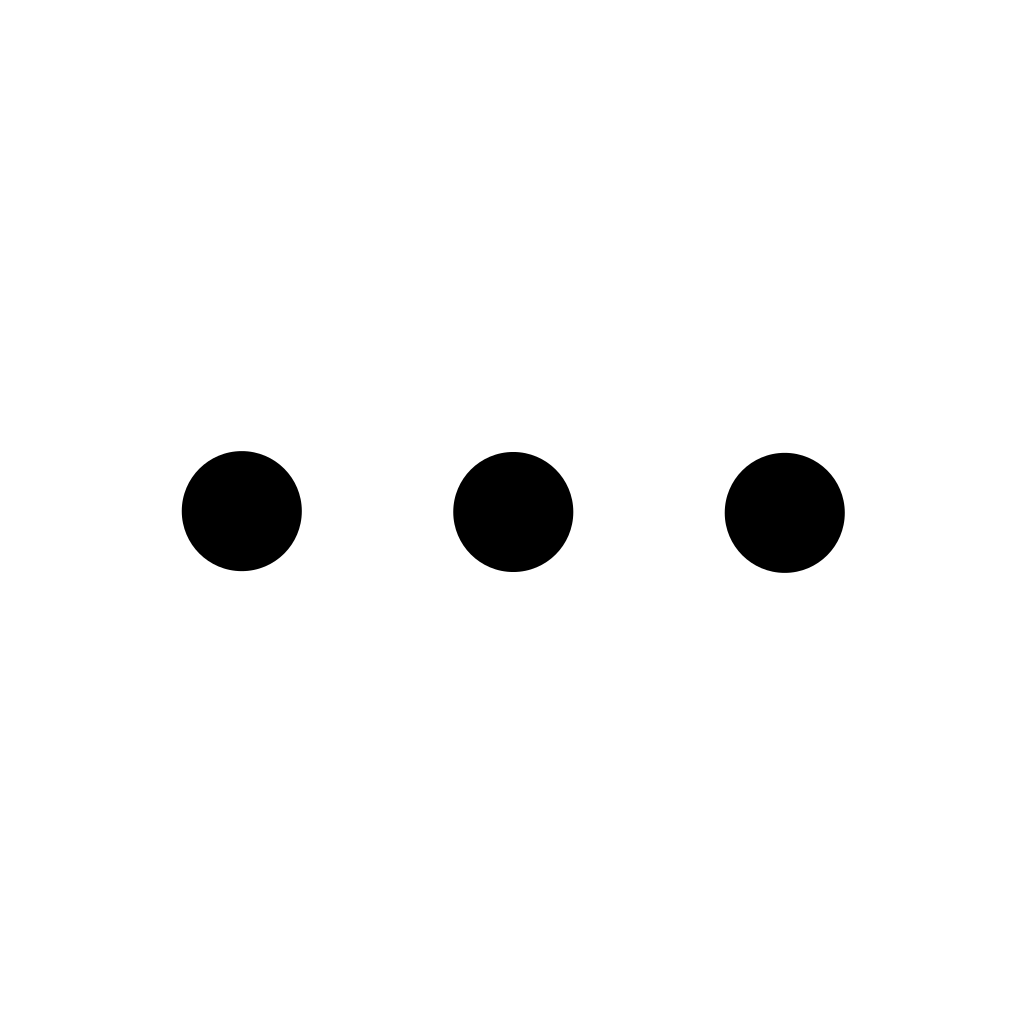
\includegraphics[width=2cm,height=2cm]{../cellipsis.png}};
%%%%%%%%%%%%%%%%%%%%%%%%%%%%%%%%%%%%%%%%%%%%%%%%%%%%%%%%%%%%%%%%%%%%%%%%%%%%%%%%%%%%%%%%
%% Linear Layer1和Linear Layer2之间的连线
%%%%%%%%%%%%%%%%%%%%%%%%%%%%%%%%%%%%%%%%%%%%%%%%%%%%%%%%%%%%%%%%%%%%%%%%%%%%%%%%%%%%%%%%
% 循环变量
\foreach \from/\to in {fc1-1-east/fc2-1-west, fc1-1-east/fc2-2-west, fc1-1-east/fc2-3-west, fc1-1-east/fc2-4-west, fc1-1-east/fc2-5-west, fc1-1-east/fc2-6-west, fc1-1-east/fc2-7-west, fc1-1-east/fc2-8-west}
    \draw[->]  (\from) -- (\to);
\foreach \from/\to in {fc1-2-east/fc2-1-west, fc1-2-east/fc2-2-west, fc1-2-east/fc2-3-west, fc1-2-east/fc2-4-west, fc1-2-east/fc2-5-west, fc1-2-east/fc2-6-west, fc1-2-east/fc2-7-west, fc1-2-east/fc2-8-west}
    \draw[->]  (\from) -- (\to);
\foreach \from/\to in {fc1-3-east/fc2-1-west, fc1-3-east/fc2-2-west, fc1-3-east/fc2-3-west, fc1-3-east/fc2-4-west, fc1-3-east/fc2-5-west, fc1-3-east/fc2-6-west, fc1-3-east/fc2-7-west, fc1-3-east/fc2-8-west}
    \draw[->]  (\from) -- (\to);
\foreach \from/\to in {fc1-4-east/fc2-1-west, fc1-4-east/fc2-2-west, fc1-4-east/fc2-3-west, fc1-4-east/fc2-4-west, fc1-4-east/fc2-5-west, fc1-4-east/fc2-6-west, fc1-4-east/fc2-7-west, fc1-4-east/fc2-8-west}
    \draw[->]  (\from) -- (\to);
\foreach \from/\to in {fc1-5-east/fc2-1-west, fc1-5-east/fc2-2-west, fc1-5-east/fc2-3-west, fc1-5-east/fc2-4-west, fc1-5-east/fc2-5-west, fc1-5-east/fc2-6-west, fc1-5-east/fc2-7-west, fc1-5-east/fc2-8-west}
    \draw[->]  (\from) -- (\to);
\foreach \from/\to in {fc1-6-east/fc2-1-west, fc1-6-east/fc2-2-west, fc1-6-east/fc2-3-west, fc1-6-east/fc2-4-west, fc1-6-east/fc2-5-west, fc1-6-east/fc2-6-west, fc1-6-east/fc2-7-west, fc1-6-east/fc2-8-west}
    \draw[->]  (\from) -- (\to);
\foreach \from/\to in {fc1-7-east/fc2-1-west, fc1-7-east/fc2-2-west, fc1-7-east/fc2-3-west, fc1-7-east/fc2-4-west, fc1-7-east/fc2-5-west, fc1-7-east/fc2-6-west, fc1-7-east/fc2-7-west, fc1-7-east/fc2-8-west}
    \draw[->]  (\from) -- (\to);
\foreach \from/\to in {fc1-8-east/fc2-1-west, fc1-8-east/fc2-2-west, fc1-8-east/fc2-3-west, fc1-8-east/fc2-4-west, fc1-8-east/fc2-5-west, fc1-8-east/fc2-6-west, fc1-8-east/fc2-7-west, fc1-8-east/fc2-8-west}
    \draw[->]  (\from) -- (\to);
\foreach \from/\to in {fc1-9-east/fc2-1-west, fc1-9-east/fc2-2-west, fc1-9-east/fc2-3-west, fc1-9-east/fc2-4-west, fc1-9-east/fc2-5-west, fc1-9-east/fc2-6-west, fc1-9-east/fc2-7-west, fc1-9-east/fc2-8-west}
    \draw[->]  (\from) -- (\to);

%%%%%%%%%%%%%%%%%%%%%%%%%%%%%%%%%%%%%%%%%%%%%%%%%%%%%%%%%%%%%%%%%%%%%%%%%%%%%%%%%%%%%%%%
%% action
%%%%%%%%%%%%%%%%%%%%%%%%%%%%%%%%%%%%%%%%%%%%%%%%%%%%%%%%%%%%%%%%%%%%%%%%%%%%%%%%%%%%%%%%
\pic[shift={(5, 0, 5)}] at (ellipsis3) {Box={name=action-value,fill=\DcColor,%
        height=3,width=3,depth=12}};
% 文字
\node[shift={(0, -1, 0)}, rotate=45] at (action-value-east) {动作分布均值};

\pic[shift={(5, 0, -5)}] at (ellipsis3) {Box={name=std-value,fill=\DcColor,%
        height=3,width=3,depth=12}};
% 文字
\node[shift={(0, -1, 0)}, rotate=45] at (std-value-east) {动作分布标准差};
%%%%%%%%%%%%%%%%%%%%%%%%%%%%%%%%%%%%%%%%%%%%%%%%%%%%%%%%%%%%%%%%%%%%%%%%%%%%%%%%%%%%%%%%
%% 输出执行动作
%%%%%%%%%%%%%%%%%%%%%%%%%%%%%%%%%%%%%%%%%%%%%%%%%%%%%%%%%%%%%%%%%%%%%%%%%%%%%%%%%%%%%%%%
% 循环变量
\foreach \from/\to in {fc2-1-east/action-value-west}
    \draw[->]  (\from) -- (\to);
\foreach \from/\to in {fc2-2-east/action-value-west}
    \draw[->]  (\from) -- (\to);
\foreach \from/\to in {fc2-3-east/action-value-west}
    \draw[->]  (\from) -- (\to);
\foreach \from/\to in {fc2-4-east/action-value-west}
    \draw[->]  (\from) -- (\to);
\foreach \from/\to in {fc2-5-east/action-value-west}
    \draw[->]  (\from) -- (\to);
\foreach \from/\to in {fc2-6-east/action-value-west}
    \draw[->]  (\from) -- (\to);
\foreach \from/\to in {fc2-7-east/action-value-west}
    \draw[->]  (\from) -- (\to);
\foreach \from/\to in {fc2-8-east/action-value-west}
    \draw[->]  (\from) -- (\to);

% 循环变量
\foreach \from/\to in {fc2-1-east/std-value-west}
    \draw[->]  (\from) -- (\to);
\foreach \from/\to in {fc2-2-east/std-value-west}
    \draw[->]  (\from) -- (\to);
\foreach \from/\to in {fc2-3-east/std-value-west}
    \draw[->]  (\from) -- (\to);
\foreach \from/\to in {fc2-4-east/std-value-west}
    \draw[->]  (\from) -- (\to);
\foreach \from/\to in {fc2-5-east/std-value-west}
    \draw[->]  (\from) -- (\to);
\foreach \from/\to in {fc2-6-east/std-value-west}
    \draw[->]  (\from) -- (\to);
\foreach \from/\to in {fc2-7-east/std-value-west}
    \draw[->]  (\from) -- (\to);
\foreach \from/\to in {fc2-8-east/std-value-west}
    \draw[->]  (\from) -- (\to);

\end{tikzpicture}
\end{document}
